\section{Other Climate Forcers}
\label{sec:other-climate-forcers}

\subsection{Well-Mixed Greenhouse Gases}
\label{sec:well-mixed-greenhouse-gases}

We have seen in previous sections that carbon dioxide is the main forcing agent of anthropogenic climate change, however,
there are severall other important players. These are are a variety of gases that are grouped into what is called the
\textbf{well-mixed greenhouse gases} (WMGHG). These are gases that are well-mixed in the atmosphere (troposphere), i.e. 
their concentrations do not vary significantly with grographical location or height. The main WMGHG are methane, CFC-11
and CFC-12.\\

Methane is the second most important anthropogenic greenhouse gas. It is emitted from a variety of sources, both natural
and anthropogenic. Its atmospheric lifetime is $\sim$12 years and it is removed from the atmosphere by reaction with the
\ce{OH} radical. Its concentration rate increase is of $\sim$18Tg\ \ce{CH4}yr$^{-1}$, i.e. emissions increase by $\sim$10\%
per decade (has been for the past two decades).\\

CFC-11 and CFC-12 are \textbf{chlorofluorocarbons} (CFCs) and are synthetic gases, part of the family of Halocarbons
(hydrocarbons that have had some or all of their hydrogen atoms replaced by halogen atoms). They are emitted from
anthropogenic sources and have lifetimes of $\sim$50 and $\sim$100 years for CFC-11 and CFC-12 respectively. 

\noindent These are inert in the troposphere but dissociate in the stratosphere leading to ozone depletion. Environmental and 
health concerns have led to the Montreal Protocol in 1987 ultimately prohibited CFC production by 2000 leading to a
decrease in their atmospheric concentrations.

\subsection{Aerosol Radiative Forcing}
\label{sec:aerosol-radiative-forcing}

Aerosols are small liquid drops or particulates suspended in the atmosphere. They can be natural or anthropogenic in
origin and can be made up of many different constituents. They can be emitted directly into the atmosphere (primary) or
formed in the atmosphere as a result of chemical processes (secondary).\\

Aerosols have a direct effect on the climate by scattering and absorbing radiation. They also have an indirect
effect by modifying the properties of clouds.

Some aerosols like black carbon or soot have a predominantly warming effect since they absorb radiation thus causing
them to warm up. More commonly, aerosols have a predominantly cooling effect since they scatter radiation back to space,
examples of this are sulphate aerosols and sea salt aerosols. It is for this reason that aerosols are believeed to have
had a cooling effect on the climate for the past 250 years or so.\\

Some aerosols like sulphate aerosols can also act as \textbf{cloud condensation nuclei} (CCN) and thus modify the 
properties of clouds. If more aerosols are present, then more CCN are present and thus more cloud droplets are formed
(smaller droplets) and thus the cloud is brighter and more reflective. This is known as the \textbf{first aerosol
indirect effect} or \textbf{Twomey effect}. 

Other indirect effects link aerosol to changes in precipitation. The smaller droplets seen above take longer to grow into
raindrops, delaying precipitation and prolonging the cloud lifetime. Both of these effects are believed to have a
cooling effect on the climate.

\begin{figure}[h]
    \centering
    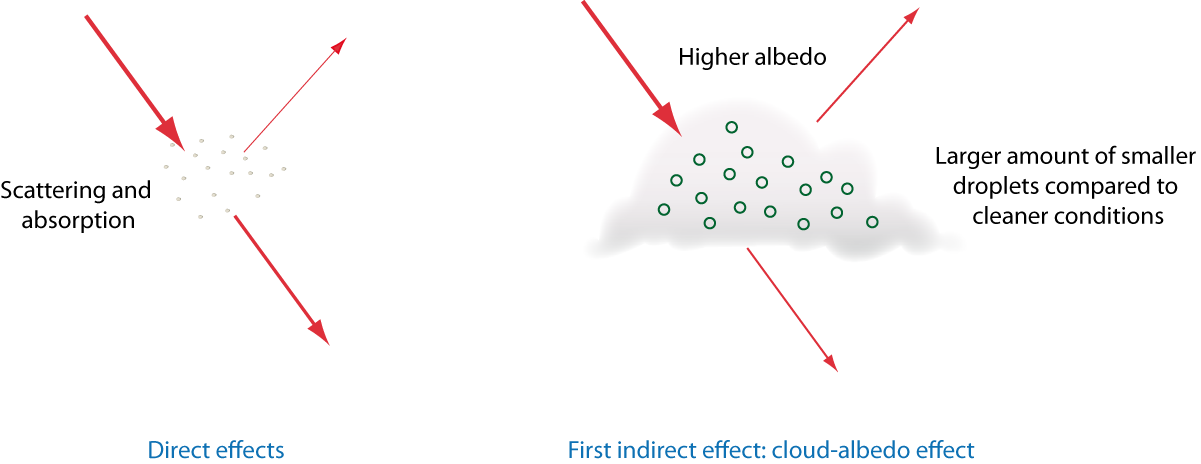
\includegraphics[width=0.8\textwidth]{figures/aerosol.png}
    \caption{Direct and indirect effects of aerosols on the climate.}
    \label{fig:aerosol}
\end{figure}

\subsection{Comparing the Impact of Different Forcing Agents}
\label{sec:comp-impact-diff}

To determine the impact a forcing agent (radiative gas or aerosol) has on the climate, we need to consider two more
things:
\begin{itemize}
    \item The lifetime of the forcing agent in the atmosphere.
    \item The radiative efficiency of the forcing agent, i.e. the ability of the forcing agent to cause a change in
    radiative forcing per unit change in concentration or amount thereof.
\end{itemize}

Hence the difficulty to compare the impact of different forcing agents without some deeper analysis. 

A metric that procides a means to compare the effectiveness of different agents to that of \ce{CO2} is the 
\textbf{Global Warming Potential} (\hyperlink{glo:global_warming_potential}{GWP}). We can define it as:
$$
\text{\hyperlink{glo:global_warming_potential}{GWP}} = \frac{\int_0^{\text{TH}} a_x[C_x(t)]dt}{\int_0^{\text{TH}} 
a_r[C_r(t)]dt}
$$
where $a_x$ is the radiative efficiency of the forcing agent $x$, $C_x(t)$ is the time-dependent concentration (decay)
of the forcing agent $x$, $a_r$ is the radiative efficiency of the reference gas (\ce{CO2}), $C_r(t)$ is the
time-dependent concentration (decay) of the reference gas (\ce{CO2}) and TH is the time horizon, or length of time over
which we evalueate the impact of the agent relative to the reference. Using \ce{CO2} as the reference gas is simply a
convention.

\begin{tcolorbox}
    \textbf{Example: Methane}\\
    We assume that we have an initial concentration of methane $C_0$ that decays exponentially with time (assumption). 
    We say that after time $\tau$ the concentration of methane has decreased by a factor of $e$ (63\%). We can then 
    caluculate the absolute GWP for methane (the numerator in the equation above) as:
    $$
    \text{AGWP}_x = \int_0^{\text{TH}} a_x[C_x(t)]dt = a_x C_{0x}\int_0^{\text{TH}} [e^{-t/\tau}]dt = 
    a_xC_{0x}\tau(1-e^{-\text{TH}/\tau})
    $$

    We note that \ce{CH4} has a radiative efficiency by \textbf{mass} of $\sim$72x that of \ce{CO2} so we write that
    $$
    a_xC_{0x} \approx 72a_rC_{0r}
    $$
    and \ce{CH4} lifetime is $\sim$12 years compared to \ce{CO2} lifetime of $\sim$200 years so we can write that the 
    global warming potential for methane is:
    $$
    \text{\hyperlink{glo:global_warming_potential}{GWP}}_{\text{CH4}} = 72\ \frac{12\left[1-e^{-\text{TH}/12}\right]}
    {200\left[1-e^{-\text{TH}/200}\right]}
    $$

    For reference we can see that in 20 years the GWP for methane is 37x that of \ce{CO2}, in 100 years it is 11x and
    500 years it is only 4.7x.
\end{tcolorbox}

This metric will be useful for policy makers to make a first order assessment of the climate impact of different
choices (e.g. changes to energy production, agricultural practices, etc.) on different timescales.
